\documentclass[border=3mm]{standalone}
\usepackage{tikz}
\usetikzlibrary{circuits.logic.US}

\begin{document}
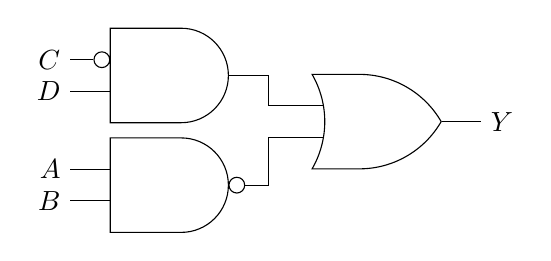
\begin{tikzpicture}[circuit logic US,
                    tiny circuit symbols,
                    every circuit symbol/.style={fill=white,draw,logic gate input sep=4mm, logic gate inverted radius=1mm}
]

\node [nand gate, inputs = nn] at (0,0) (and1) {};
\node [and gate, inputs = in] at ($(and1.south) + (0,2.0cm)$) (and2) {};
\node [or gate, inputs = nn, anchor=input 2] at ($(and1.north)+(2.0cm,0)$) (or1) {};
%
\draw (and1.input 1) -- ++(left:5mm) node[left] (A) {$A$};
\draw (and1.input 2) -- ++(left:5mm) node[left] {$B$};
%\node (C) at (A|-or1.input 2) {$C$};
%\draw (or1.input 1) -- (C);
\draw (and1.output) -- ++(right:3mm) |- (or1.input 2);
\draw (or1.output) -- ++(right:5mm) node[right] (Y) {$Y$};
%
\draw (and2.input 1) -- ++(left:3mm) node[left] (C) {$C$};
\draw (and2.input 2) -- ++(left:5mm) node[left] (D) {$D$};
\draw (and2.output) -- ++(right:5mm) |- (or1.input 1);
\end{tikzpicture}
\end{document}
